% Standalone preview of the Module 1 frames. Compile with pdflatex.
% In the main deck, only % ======================================================================
% Module 1: motivation, SEIRD model, published models, phase plane
% Three frames, no title slide: \input this file into the main deck.
%
% Needs in the main preamble:  \usepackage{graphicx,booktabs,amssymb,tikz}
%                              \usetikzlibrary{arrows.meta,positioning}
% Figures are in figs/ next to this file. If this file sits in a folder
% (e.g. module1/), add \graphicspath{{module1/}} to the main preamble.
% All numbers are from report/main.tex (final Colab run).
% ======================================================================

% Shared deck colours (same values as Module 5)
\definecolor{mvPINN}{HTML}{7B2D8E}
\definecolor{mvInk}{HTML}{1F2933}
\definecolor{mvMuted}{HTML}{5F6B7A}
\definecolor{mvSoft}{HTML}{F3EDF6}
\definecolor{mvRule}{HTML}{C9B6D3}
% Model colours match the published-models figure
\definecolor{moStatic}{HTML}{1F77B4}
\definecolor{moAlthaus}{HTML}{D62728}
\definecolor{moRivers}{HTML}{2CA02C}
\definecolor{moDynamic}{HTML}{9333EA}

\providecommand{\mvTakeaway}[1]{%
  \par\vspace{3pt}\noindent
  \fcolorbox{mvRule}{mvSoft}{\parbox{\dimexpr\linewidth-2\fboxsep-2\fboxrule\relax}{\footnotesize\color{mvInk}#1}}}

% ----------------------------------------------------------------------
\begin{frame}{Why transmission must change over time}
\framesubtitle{Module 1 \textbullet\ Ebola in Sierra Leone, 2014--15 \textbullet\ an SEIRD model with a time-varying transmission rate $\beta(t)$}
\vspace{-2pt}
\begin{columns}[T,onlytextwidth]
\column{0.52\textwidth}
  \footnotesize\raggedright
  \textbf{\color{mvPINN}The problem}
  \begin{itemize}\setlength{\itemsep}{1pt}
    \item Ebola spreads by contact with body fluids, and with the dead at funerals
    \item isolation, safe burials and contact tracing cut transmission as the epidemic went on: $\beta$ is \textbf{not} a constant
    \item surveillance reports only cases and deaths; $S$ and $E$ are never measured
  \end{itemize}
  \vspace{4pt}
  \centering
  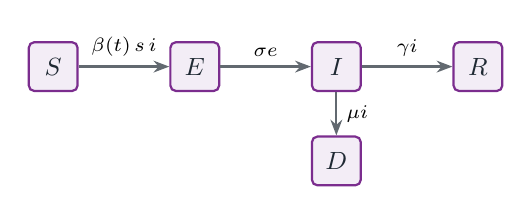
\begin{tikzpicture}[
      node distance=1.15cm,
      box/.style={rectangle, draw=mvPINN, fill=mvSoft, thick, minimum size=0.62cm,
                  font=\bfseries\small, rounded corners=2pt, text=mvInk},
      arr/.style={-{Stealth[length=2mm]}, thick, draw=mvInk!70}]
    \node[box] (S) {$S$};
    \node[box, right=of S] (E) {$E$};
    \node[box, right=of E] (I) {$I$};
    \node[box, right=of I] (R) {$R$};
    \node[box, below=0.55cm of I] (D) {$D$};
    \draw[arr] (S) -- node[above, font=\scriptsize] {$\beta(t)\,s\,i$} (E);
    \draw[arr] (E) -- node[above, font=\scriptsize] {$\sigma e$} (I);
    \draw[arr] (I) -- node[above, font=\scriptsize] {$\gamma i$} (R);
    \draw[arr] (I) -- node[right, font=\scriptsize] {$\mu i$} (D);
  \end{tikzpicture}\\[3pt]
  {\scriptsize $\dot s = -\beta s i,\;\; \dot e = \beta s i - \sigma e,\;\; \dot i = \sigma e - (\gamma+\mu) i,\;\; \dot r = \gamma i,\;\; \dot d = \mu i$\\[1pt]
  fractions of $N$, so $s+e+i+r+d = 1$ at all times}
\column{0.44\textwidth}
  \scriptsize\setlength{\tabcolsep}{4pt}
  \begin{tabular}{@{}lll@{}}
    \toprule
    & Meaning & Value \\
    \midrule
    $N$      & population (2014 census)  & 7{,}092{,}113 \\
    $\sigma$ & incubation rate (9.4 days) & 0.1064 /day \\
    $\gamma$ & recovery rate (7 days)     & 0.1429 /day \\
    $\mu$    & death rate                 & 0.1000 /day \\
    $\beta$  & transmission rate (baseline) & 0.4858 /day \\
    \midrule
    CFR      & $\mu/(\gamma+\mu)$          & 41.2\% \\
    $R_0$    & $\beta/(\gamma+\mu)$        & 2.00 \\
    \bottomrule
  \end{tabular}\\[5pt]
  \footnotesize
  \textbf{\color{mvPINN}Assumptions}
  \begin{itemize}\setlength{\itemsep}{0pt}
    \item closed population, homogeneous mixing
    \item recovered people stay immune
    \item $\sigma,\gamma$ fixed from WHO clinical data, so the data only have to determine $\beta(t)$ and $\mu$
  \end{itemize}
\end{columns}
\mvTakeaway{\textbf{Why $\beta(t)$:} with a constant $\beta$ ($R_0 = 2$) the model predicts about \textbf{80\%} of Sierra Leone infected and \textbf{33\%} dead.
WHO confirmed 8{,}704 cases, about \textbf{0.12\%}. The difference is that transmission fell.}
\end{frame}

% ----------------------------------------------------------------------
\begin{frame}{Published models: how others handled $\beta(t)$}
\framesubtitle{Module 1 \textbullet\ each makes one assumption about how transmission changes \textbullet\ figure: illustrative shapes over 120 days}
\vspace{-2pt}
\begin{columns}[T,onlytextwidth]
\column{0.48\textwidth}
  \centering
  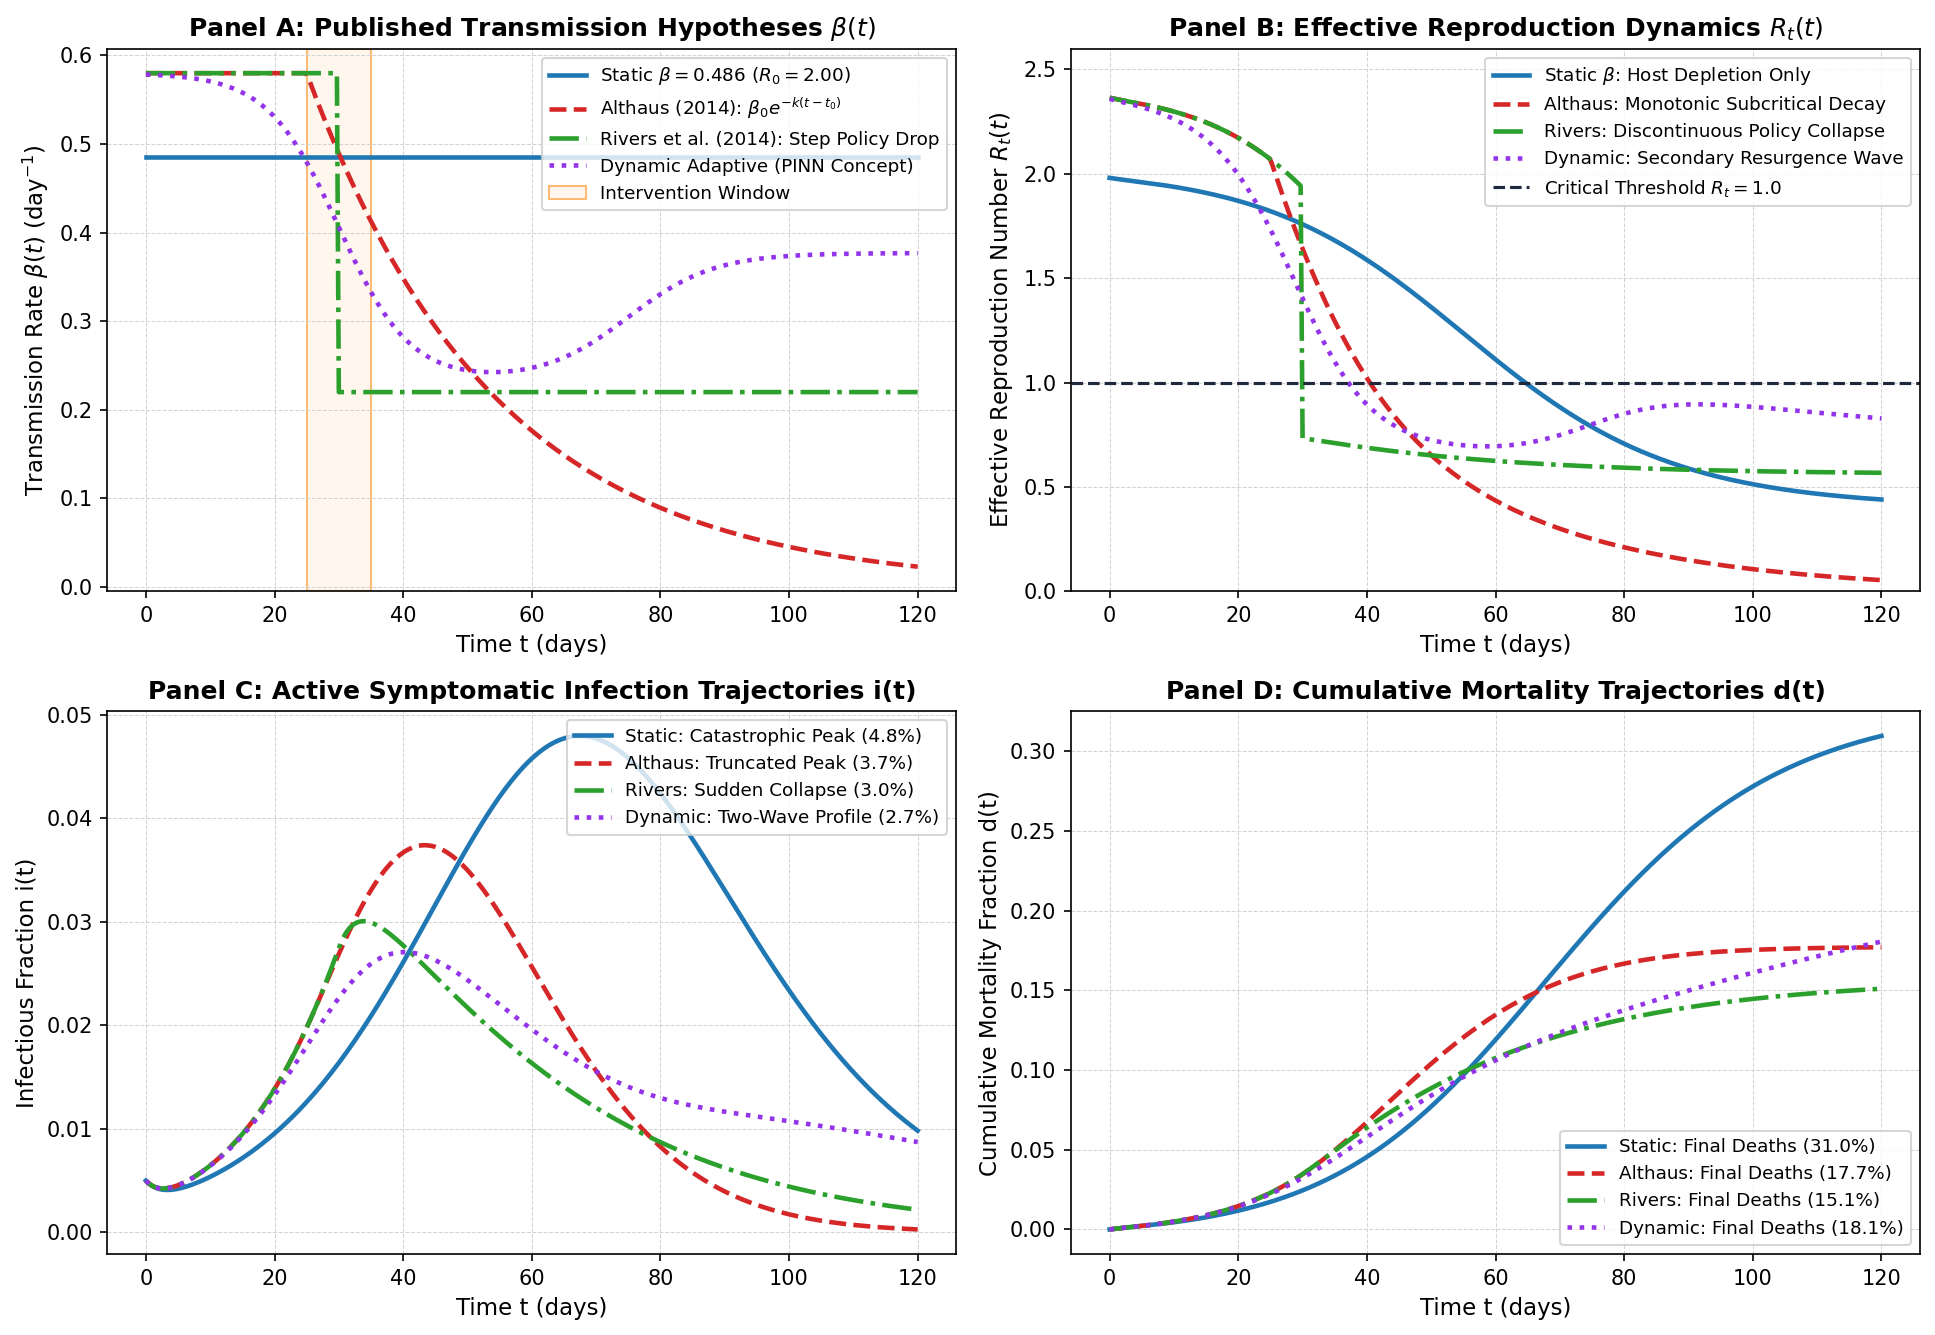
\includegraphics[width=\linewidth]{figs/m1_published_models.png}
\column{0.50\textwidth}
  \scriptsize\setlength{\tabcolsep}{2.5pt}
  \begin{tabular}{@{}lll@{}}
    \toprule
    Model & $\beta(t)$ & Limitation \\
    \midrule
    \textbf{Chowell} (2004) & drops after control starts & shape assumed \\
    \textbf{Legrand} (2007) & 3 routes: $\beta_I, \beta_H, \beta_F$ & routes not separable \\
    \textbf{\color{moRivers}Rivers} (2014) & step at a policy date & abrupt; date assumed \\
    \textbf{\color{moAlthaus}Althaus} (2014) & $\beta_0 e^{-k(t-t_0)}$ & can only fall \\
    \midrule
    \textbf{\color{mvPINN}Our PINN} & learned from data & smooth, any shape \\
    \bottomrule
  \end{tabular}\\[2pt]
  {\tiny\color{mvMuted} Legrand: from one national case curve the three routes trade off against each other.}\\[4pt]
  \footnotesize
  \textbf{\color{moAlthaus}Althaus, in one line:}
  \[ \frac{dR_t}{dt} = -\frac{\beta s}{\gamma+\mu}\,\big[k + \beta i\big] < 0 \]
  so once $R_t < 1$ it can never rise again.
\end{columns}
\mvTakeaway{\textbf{The gap:} every published model fixes the \emph{shape} of $\beta(t)$ in advance (a date, a step, a decay).
Our PINN learns $\beta(t)$ from cases and deaths, with no date or shape assumed.}
\end{frame}

% ----------------------------------------------------------------------
\begin{frame}{Phase plane: the peak and the control threshold}
\framesubtitle{Module 1 \textbullet\ exact formulas, checked against an accurate ODE solver (DOP853)}
\vspace{-2pt}
\begin{columns}[T,onlytextwidth]
\column{0.50\textwidth}
  \centering
  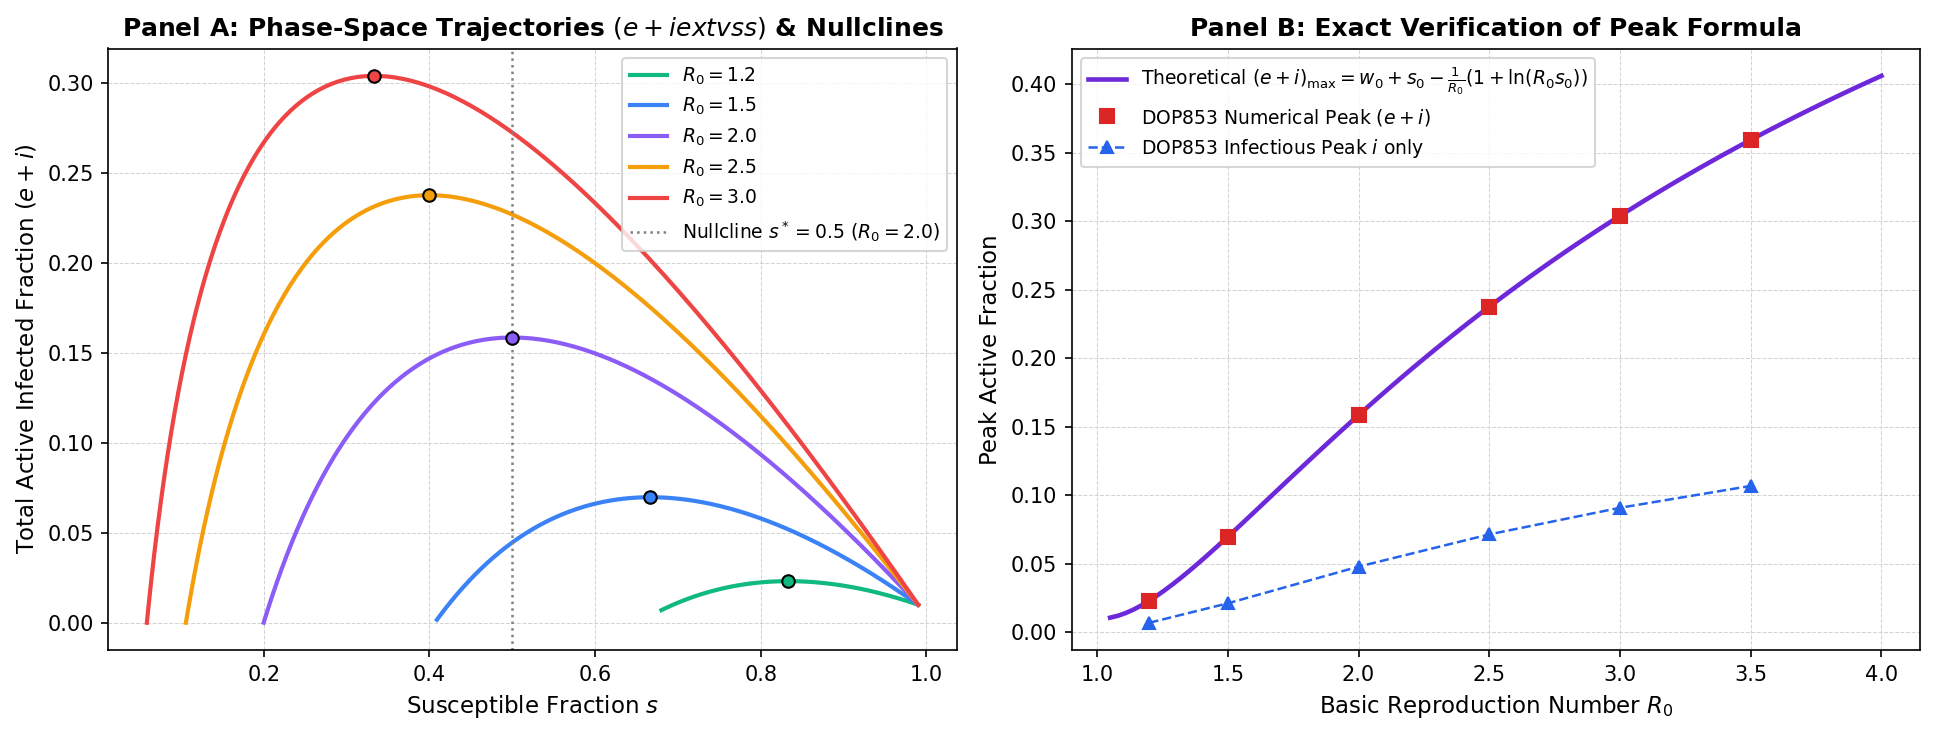
\includegraphics[height=0.56\textheight,trim=0 0 470 24,clip]{figs/m1_phase_space.png}\\[1pt]
  {\scriptsize\color{mvMuted} $R_0 = 1.2$--$3.0$; time runs right to left; dots = predicted peaks}
\column{0.47\textwidth}
  \footnotesize\raggedright
  \textbf{\color{mvPINN}Divide the equations: $i$ cancels exactly}
  \[ \frac{d(e+i)}{ds} = -1 + \frac{1}{R_0\, s} \]
  \textbf{\color{mvPINN}Peak} where the slope is zero: $s^* = 1/R_0$
  \[ (e+i)_{\max} = (e_0+i_0) + s_0 - \tfrac{1}{R_0}\big[1 + \ln(R_0 s_0)\big] \]
  \vspace{-4pt}
  \begin{itemize}\setlength{\itemsep}{1pt}
    \item $R_0 = 2$: peak \textbf{15.85\%} at $s = 0.5$ ($i$ alone about 4.8\%)
    \item formula vs.\ ODE: relative error at most $1.3\times10^{-5}$
  \end{itemize}
  \vspace{2pt}
  \textbf{\color{mvPINN}Control threshold}
  \[ p_c = \delta_c = 1 - \frac{1}{R_0} = 50\% \quad (R_0 = 2) \]
\end{columns}
\mvTakeaway{\textbf{What it means for control:} without a vaccine, isolation, safe burials and tracing together must cut transmission by \textbf{more than 50\%} to turn the epidemic.
These exact formulas are also the checks used for the solvers (Module 3) and the PINN (Module 4).}
\end{frame}
 is needed.
\documentclass[aspectratio=169,10pt]{beamer}
\usepackage{graphicx,booktabs,amssymb}
\usepackage{tikz}
\usetikzlibrary{arrows.meta,positioning}

\usetheme{default}
\setbeamertemplate{navigation symbols}{}
\definecolor{deckInk}{HTML}{1F2933}
\definecolor{deckAccent}{HTML}{7B2D8E}
\setbeamercolor{frametitle}{fg=deckInk}
\setbeamercolor{framesubtitle}{fg=deckInk!60}
\setbeamercolor{structure}{fg=deckAccent}
\setbeamerfont{frametitle}{series=\bfseries,size=\large}
\setbeamerfont{framesubtitle}{size=\scriptsize}
\setbeamertemplate{frametitle}{%
  \vspace*{4pt}\insertframetitle\par
  {\usebeamerfont{framesubtitle}\usebeamercolor[fg]{framesubtitle}\insertframesubtitle\par}
  \vskip3pt{\color{deckAccent}\hrule height 0.6pt}\vskip-4pt}
\setbeamertemplate{footline}{\hfill{\scriptsize\color{deckInk!50}\insertframenumber}\hspace*{10pt}\vspace*{6pt}}
\setbeamersize{text margin left=18pt,text margin right=18pt}

\begin{document}
% ======================================================================
% Module 1: motivation, SEIRD model, published models, phase plane
% Three frames, no title slide: \input this file into the main deck.
%
% Needs in the main preamble:  \usepackage{graphicx,booktabs,amssymb,tikz}
%                              \usetikzlibrary{arrows.meta,positioning}
% Figures are in figs/ next to this file. If this file sits in a folder
% (e.g. module1/), add \graphicspath{{module1/}} to the main preamble.
% All numbers are from report/main.tex (final Colab run).
% ======================================================================

% Shared deck colours (same values as Module 5)
\definecolor{mvPINN}{HTML}{7B2D8E}
\definecolor{mvInk}{HTML}{1F2933}
\definecolor{mvMuted}{HTML}{5F6B7A}
\definecolor{mvSoft}{HTML}{F3EDF6}
\definecolor{mvRule}{HTML}{C9B6D3}
% Model colours match the published-models figure
\definecolor{moStatic}{HTML}{1F77B4}
\definecolor{moAlthaus}{HTML}{D62728}
\definecolor{moRivers}{HTML}{2CA02C}
\definecolor{moDynamic}{HTML}{9333EA}

\providecommand{\mvTakeaway}[1]{%
  \par\vspace{3pt}\noindent
  \fcolorbox{mvRule}{mvSoft}{\parbox{\dimexpr\linewidth-2\fboxsep-2\fboxrule\relax}{\footnotesize\color{mvInk}#1}}}

% ----------------------------------------------------------------------
\begin{frame}{Why transmission must change over time}
\framesubtitle{Module 1 \textbullet\ Ebola in Sierra Leone, 2014--15 \textbullet\ an SEIRD model with a time-varying transmission rate $\beta(t)$}
\vspace{-2pt}
\begin{columns}[T,onlytextwidth]
\column{0.52\textwidth}
  \footnotesize\raggedright
  \textbf{\color{mvPINN}The problem}
  \begin{itemize}\setlength{\itemsep}{1pt}
    \item Ebola spreads by contact with body fluids, and with the dead at funerals
    \item isolation, safe burials and contact tracing cut transmission as the epidemic went on: $\beta$ is \textbf{not} a constant
    \item surveillance reports only cases and deaths; $S$ and $E$ are never measured
  \end{itemize}
  \vspace{4pt}
  \centering
  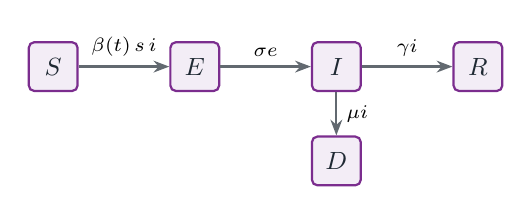
\begin{tikzpicture}[
      node distance=1.15cm,
      box/.style={rectangle, draw=mvPINN, fill=mvSoft, thick, minimum size=0.62cm,
                  font=\bfseries\small, rounded corners=2pt, text=mvInk},
      arr/.style={-{Stealth[length=2mm]}, thick, draw=mvInk!70}]
    \node[box] (S) {$S$};
    \node[box, right=of S] (E) {$E$};
    \node[box, right=of E] (I) {$I$};
    \node[box, right=of I] (R) {$R$};
    \node[box, below=0.55cm of I] (D) {$D$};
    \draw[arr] (S) -- node[above, font=\scriptsize] {$\beta(t)\,s\,i$} (E);
    \draw[arr] (E) -- node[above, font=\scriptsize] {$\sigma e$} (I);
    \draw[arr] (I) -- node[above, font=\scriptsize] {$\gamma i$} (R);
    \draw[arr] (I) -- node[right, font=\scriptsize] {$\mu i$} (D);
  \end{tikzpicture}\\[3pt]
  {\scriptsize $\dot s = -\beta s i,\;\; \dot e = \beta s i - \sigma e,\;\; \dot i = \sigma e - (\gamma+\mu) i,\;\; \dot r = \gamma i,\;\; \dot d = \mu i$\\[1pt]
  fractions of $N$, so $s+e+i+r+d = 1$ at all times}
\column{0.44\textwidth}
  \scriptsize\setlength{\tabcolsep}{4pt}
  \begin{tabular}{@{}lll@{}}
    \toprule
    & Meaning & Value \\
    \midrule
    $N$      & population (2014 census)  & 7{,}092{,}113 \\
    $\sigma$ & incubation rate (9.4 days) & 0.1064 /day \\
    $\gamma$ & recovery rate (7 days)     & 0.1429 /day \\
    $\mu$    & death rate                 & 0.1000 /day \\
    $\beta$  & transmission rate (baseline) & 0.4858 /day \\
    \midrule
    CFR      & $\mu/(\gamma+\mu)$          & 41.2\% \\
    $R_0$    & $\beta/(\gamma+\mu)$        & 2.00 \\
    \bottomrule
  \end{tabular}\\[5pt]
  \footnotesize
  \textbf{\color{mvPINN}Assumptions}
  \begin{itemize}\setlength{\itemsep}{0pt}
    \item closed population, homogeneous mixing
    \item recovered people stay immune
    \item $\sigma,\gamma$ fixed from WHO clinical data, so the data only have to determine $\beta(t)$ and $\mu$
  \end{itemize}
\end{columns}
\mvTakeaway{\textbf{Why $\beta(t)$:} with a constant $\beta$ ($R_0 = 2$) the model predicts about \textbf{80\%} of Sierra Leone infected and \textbf{33\%} dead.
WHO confirmed 8{,}704 cases, about \textbf{0.12\%}. The difference is that transmission fell.}
\end{frame}

% ----------------------------------------------------------------------
\begin{frame}{Published models: how others handled $\beta(t)$}
\framesubtitle{Module 1 \textbullet\ each makes one assumption about how transmission changes \textbullet\ figure: illustrative shapes over 120 days}
\vspace{-2pt}
\begin{columns}[T,onlytextwidth]
\column{0.48\textwidth}
  \centering
  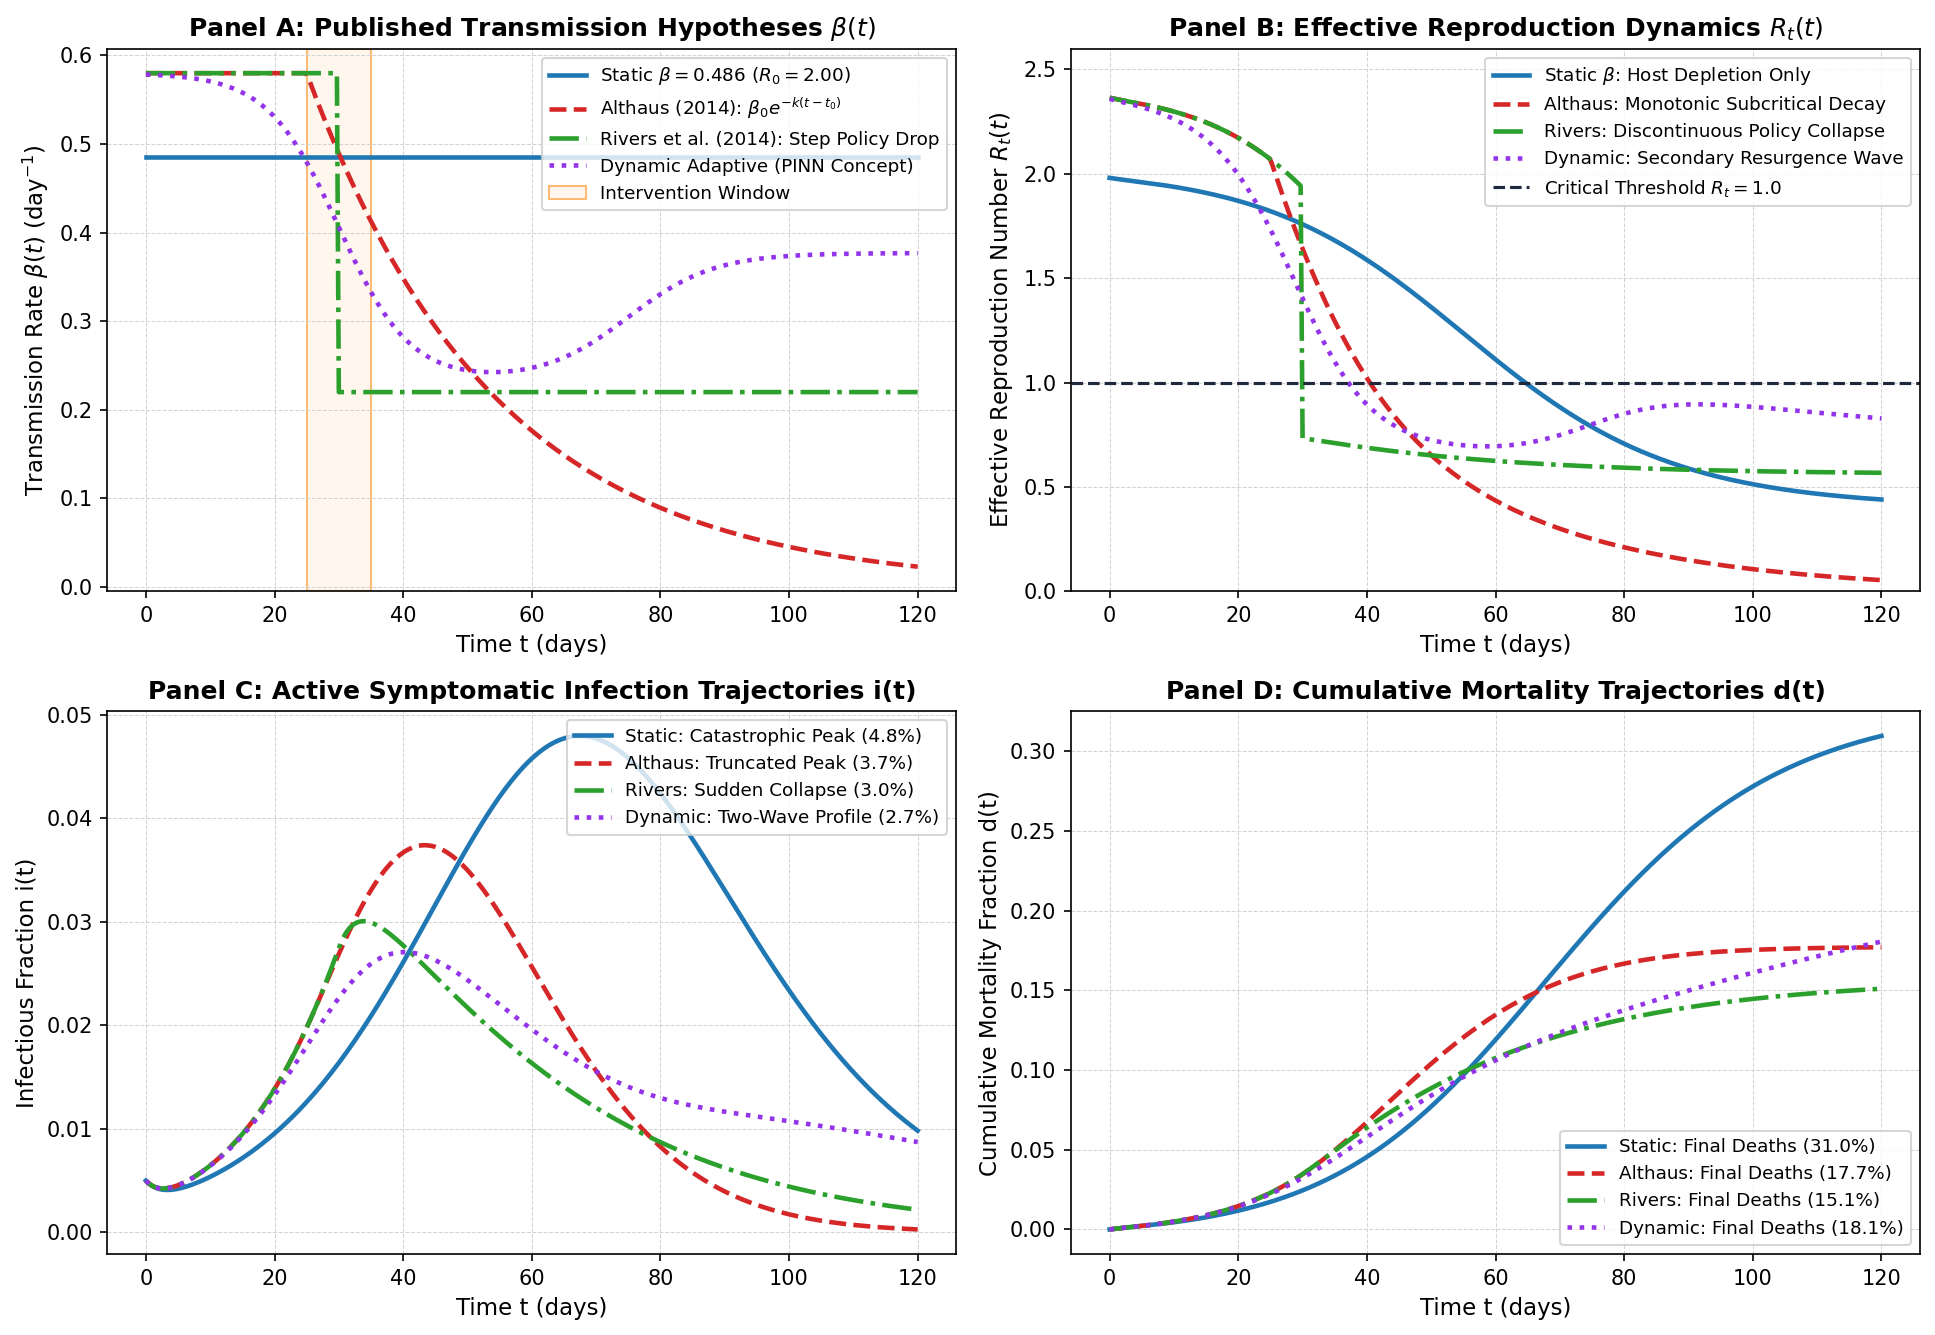
\includegraphics[width=\linewidth]{figs/m1_published_models.png}
\column{0.50\textwidth}
  \scriptsize\setlength{\tabcolsep}{2.5pt}
  \begin{tabular}{@{}lll@{}}
    \toprule
    Model & $\beta(t)$ & Limitation \\
    \midrule
    \textbf{Chowell} (2004) & drops after control starts & shape assumed \\
    \textbf{Legrand} (2007) & 3 routes: $\beta_I, \beta_H, \beta_F$ & routes not separable \\
    \textbf{\color{moRivers}Rivers} (2014) & step at a policy date & abrupt; date assumed \\
    \textbf{\color{moAlthaus}Althaus} (2014) & $\beta_0 e^{-k(t-t_0)}$ & can only fall \\
    \midrule
    \textbf{\color{mvPINN}Our PINN} & learned from data & smooth, any shape \\
    \bottomrule
  \end{tabular}\\[2pt]
  {\tiny\color{mvMuted} Legrand: from one national case curve the three routes trade off against each other.}\\[4pt]
  \footnotesize
  \textbf{\color{moAlthaus}Althaus, in one line:}
  \[ \frac{dR_t}{dt} = -\frac{\beta s}{\gamma+\mu}\,\big[k + \beta i\big] < 0 \]
  so once $R_t < 1$ it can never rise again.
\end{columns}
\mvTakeaway{\textbf{The gap:} every published model fixes the \emph{shape} of $\beta(t)$ in advance (a date, a step, a decay).
Our PINN learns $\beta(t)$ from cases and deaths, with no date or shape assumed.}
\end{frame}

% ----------------------------------------------------------------------
\begin{frame}{Phase plane: the peak and the control threshold}
\framesubtitle{Module 1 \textbullet\ exact formulas, checked against an accurate ODE solver (DOP853)}
\vspace{-2pt}
\begin{columns}[T,onlytextwidth]
\column{0.50\textwidth}
  \centering
  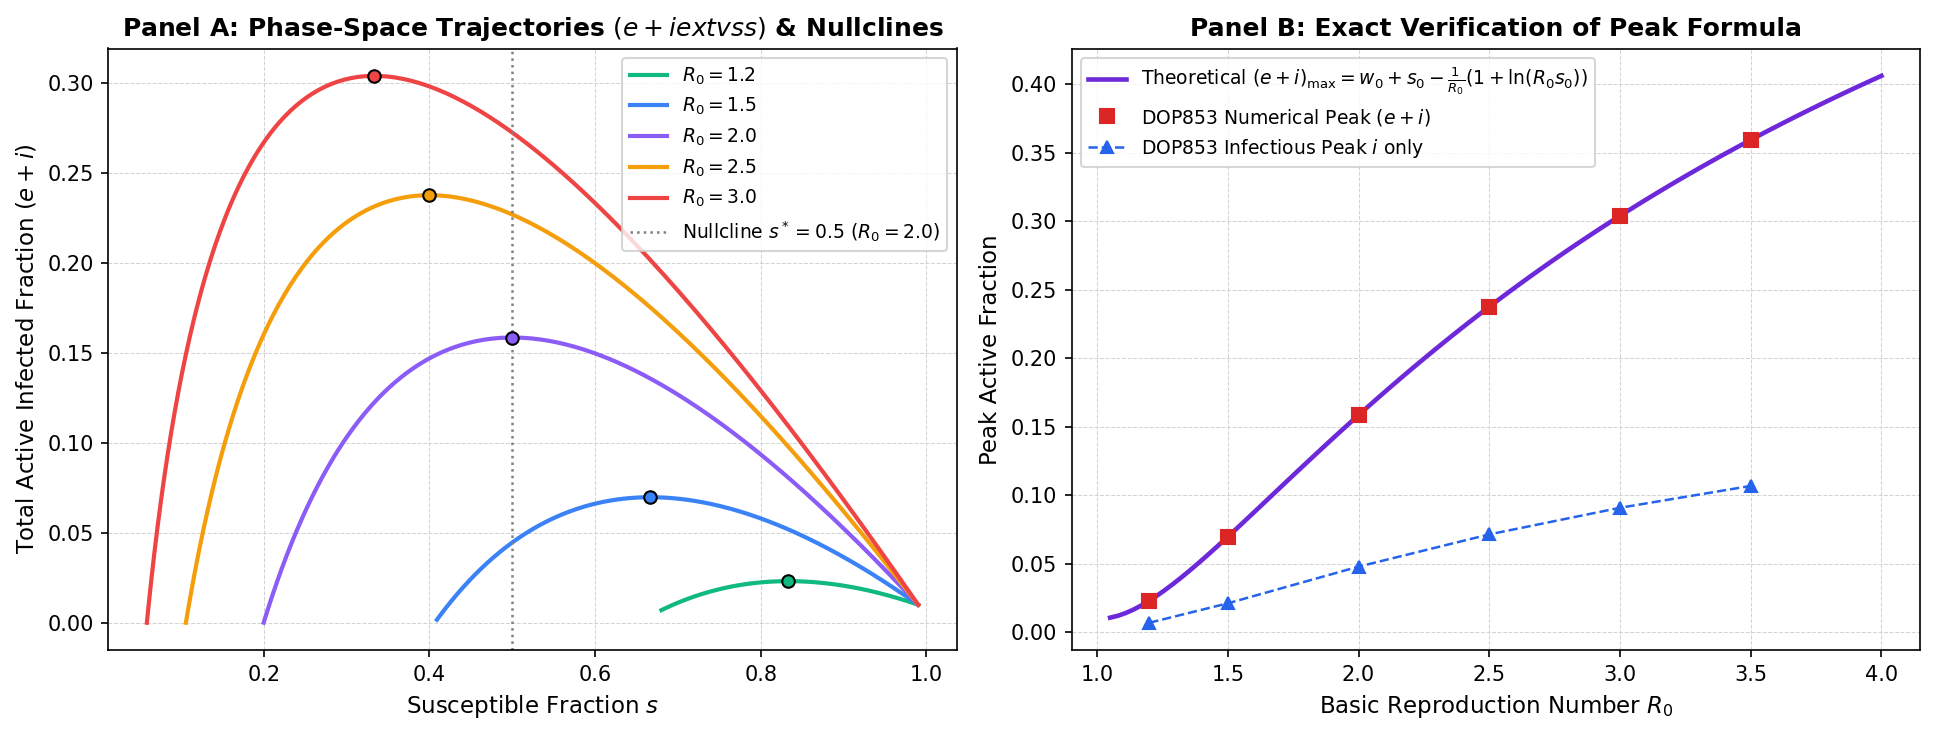
\includegraphics[height=0.56\textheight,trim=0 0 470 24,clip]{figs/m1_phase_space.png}\\[1pt]
  {\scriptsize\color{mvMuted} $R_0 = 1.2$--$3.0$; time runs right to left; dots = predicted peaks}
\column{0.47\textwidth}
  \footnotesize\raggedright
  \textbf{\color{mvPINN}Divide the equations: $i$ cancels exactly}
  \[ \frac{d(e+i)}{ds} = -1 + \frac{1}{R_0\, s} \]
  \textbf{\color{mvPINN}Peak} where the slope is zero: $s^* = 1/R_0$
  \[ (e+i)_{\max} = (e_0+i_0) + s_0 - \tfrac{1}{R_0}\big[1 + \ln(R_0 s_0)\big] \]
  \vspace{-4pt}
  \begin{itemize}\setlength{\itemsep}{1pt}
    \item $R_0 = 2$: peak \textbf{15.85\%} at $s = 0.5$ ($i$ alone about 4.8\%)
    \item formula vs.\ ODE: relative error at most $1.3\times10^{-5}$
  \end{itemize}
  \vspace{2pt}
  \textbf{\color{mvPINN}Control threshold}
  \[ p_c = \delta_c = 1 - \frac{1}{R_0} = 50\% \quad (R_0 = 2) \]
\end{columns}
\mvTakeaway{\textbf{What it means for control:} without a vaccine, isolation, safe burials and tracing together must cut transmission by \textbf{more than 50\%} to turn the epidemic.
These exact formulas are also the checks used for the solvers (Module 3) and the PINN (Module 4).}
\end{frame}

\end{document}
